%\documentclass[german,bachelor]{webisthesis}
\documentclass[english,bachelor]{webisthesis}
% When you change the language, pdflatex may halt on recompilation.
% Just hit enter to continue and recompile again. This should fix it.

%
% Values
% ------
\ThesisSetTitle{On the Viability of Phonetic Transcriptions for Authorship Verification}
\ThesisSetKeywords{Authorship Verification, Phonetic Transcription} % only for PDF meta attributes

\ThesisSetAuthor{David Reinartz}
\ThesisSetStudentNumber{3706997}
\ThesisSetDateOfBirth{2}{5}{1998}
\ThesisSetPlaceOfBirth{Ostercappeln}

\ThesisSetSupervisors{Prof.\ Dr.\ Martin Potthast,Prof.\ Dr.\ Benno Stein}

\ThesisSetSubmissionDate{4}{8}{2021}

%
% Suggested Packages
% ------------------
\usepackage[sort&compress]{natbib}
%   Allows citing in different ways (e.g., only the authors if you use the
%   citation again within a short time).
%
\usepackage{booktabs}
%    For tables ``looking the right way''.
%
\usepackage{tabularx}
%    Enables tables with columns that automatically fill the page width.
%
%\usepackage[ruled,algochapter]{algorithm2e}
%    A package for pseudo code algorithms.
%
\usepackage{amsmath}
%    For tabular-style formatting of mathematical environments.
%

%
% Commenting (by your supervisor)
% -------------------------------
\usepackage{xcolor}
\usepackage{soul}
\usepackage{amssymb}
\usepackage{svg}
%\setsvg{inkscape=inkscape -z -D,svgpath=figures/}
%\usepackage[clean]{svg}
\usepackage{tipa}
\usepackage{graphicx}
\newcommand{\bscom}[2]{%
  % #1 Original text.
  % #2 Replacement text.
    \st{\scriptsize\,#1}{\color{blue}\scriptsize\,#2}%
  }

% Create links in the pdf document
% Hyperref has some incompatibilities with other packages
% Some other packages must be loaded before, some after hyperref
% Additional options to the hyperref package can be provided in the braces []
\usehyperref[backref] % This will add back references in the bibliography

% \specialcell can be used for multiline cell in table
\newcommand{\specialcell}[2][c]{%
  \begin{tabular}[#1]{@{}c@{}}#2\end{tabular}}

% Make floating figures only get a separate page when they occupy more than
% 80% of the page, default = 60%.
\renewcommand{\floatpagefraction}{.8}%

\begin{document}
\begin{frontmatter}
\begin{abstract}
% Make textwidth smaller
(Note: very early version, will change.)
Authorship Verification is an important task in the field of stylometry.
We hypothesize that an author has a certain phonetic preference which leads them to unconsciously imprint (latent) features into written text.
Using a range of phonetic transcription systems in conjunction with two well-known Authorship Verification algorithms, we examine the use of extracting phonetically relevant features in Authorship Verification.
We find that the benefits of using these transcription systems is insignificant.
We point out that there are two major problems in this approach which need further investigation.
For reproducibility, all code is published as open-source.
\end{abstract}
  \tableofcontents
  \thispagestyle{empty}

  %\chapter*{Acknowledgements} % optional
  %I thank the authors of the webisthesis template for their excellent work!

  %\listoffigures % optional

  %\listoftables % optional

  %\listofalgorithms % optional
  %    requires package algorithm2e

  % optional: list of symbols/notation (e.g., using the nomencl package)

\end{frontmatter}

\chapter{Introduction}\label{introduction}
With the widespread availability and use of text as a medium of information transfer, the problem of identifying authorship of given texts has become one of the main focuses of stylometric analysis.
In this paper, we specifically tackle the task of Authorship Verification which consists of classifying whether two given texts were written by the same author or not.
Underlying our approach is the hypothesis that authors have a \textit{phonetic preference}, based on which they produce different texts.
\cite{ladefoged2014courseInPhonetics} titles this preference the ``phonetics of the individual'' and states that ``[...] the set of phonetic habits and memories that each speaker possesses is different from those of every other speaker of the language''.
By applying phonetic transcription systems of varied granularity to the data used, we aim to emphasize these phonetically relevant features implanted into the texts by their authors.
Then, we use the transcribed data to train two well-known Authorship Verification classifiers.
By evaluating the results with standard measures used in Authorship Verification, we aim to answer the following questions:
\begin{itemize}
  \item Does the prior phonetic transcription of texts improve the performance of the algorithms over using verbatim text?
  \item Are the results correlated to the granularities of the transcriptions?
\end{itemize}
We transcribe textual data to North American English pronunciation.
We are aware that in this process some author-specific information is lost and will discuss the implications of this.
Nevertheless, we anticipate that the phonetic information encoded into plain text and boosted by transcribing gives the classifiers an advantage over more na\"{\i}ve methods.
All code attributions are open-sourced at \url{https://github.com/torond/bachelors-thesis} with an emphasis on ease of reproduction.


% % Showing natbib citation commands
% Let us get started by citing \citet{manning:1999}!
% So what did \citeauthor{manning:1999} do in % \citeyear{manning:1999}?
% Good question!
% % Showing hyperref reference commands
% Maybe it is answered in \autoref{introduction} on % page~\pageref{introduction}?
% Just to have something show up in the list of figures, I % included \autoref{fig:a}.
% \begin{figure}[bt]% bottom or top of page (for small % figures/tables)
%   \begin{center}{\huge\bf A}\end{center}
%   \caption{The first letter in the Roman % alphabet.}\label{fig:a}
% \end{figure}
% % \formatdate (or \formatdateshort)
% This date does not exist: \formatdateshort{30}{2}{2014}
% and is the same as \formatdate{30}{2}{2014}.
% % An example table
% And here is some table with some numbers % (\autoref{tab:numbers})
% which deserves to be on an extra page.
% \begin{table}[p]% extra page (usually for large figures/tables)
%   \caption{Tables have their captions above, figures below.}
%   \begin{center}
%     \begin{tabular}{lccc}\toprule
%       \multicolumn{4}{c}{Some numbers}\\\midrule
%       & 1999 & 2000 & 2001 \\\cmidrule(l){2-4}
%       % cmidrule: A line from 2nd to 4th column, trimmed on the % left hand side
%       Distance (km) & 23 & 18 & 42 \\
%       Awesomeness (aws) & 3.2 & 8.1 & 2.4 \\\bottomrule
%     \end{tabular}
%   \end{center}\label{tab:numbers}%
% \end{table}
\chapter{Background}\label{ch:background}
% Authorship Verification
\section{Authorship Verification}\label{sec:authorship-verification}
In our world a large amount of communication and information transfer is done through a visual medium: text.
This was not always the case.
According to \cite{owidliteracy}, for most of history, reading and writing was reserved to an elite and associated with power.
Through the spread of public education over time, increasingly more people were able to read and write.
World-wide literacy rates are estimated to have been at 12\% in 1820 and have risen to 86\% in 2016.
\cite{buringh2009charting} estimates that the number of books produced annually in Western Europe in the sixth and seventh centuries was only around 120.
In contrast, and not only due to the invention of letterpress printing with movable type, the production in 1790 was at a peak of 20,000,000 books per year.
These historical processes gave rise to the linguistic branch of Stylometry, the analysis of ``an author's work based especially on the recurrence of particular turns of expression or trends of thought''\footnote{\url{https://www.merriam-webster.com/dictionary/stylometry}}.
The worth of profiling authors can be illustrated with an anecdote about a court case from 1979 published in \cite{hitt2012shuyCase}.
The American linguist Roger Shuy was able to infer that the author of a ransom note linked to a kidnapping case had to be well-educated and from Akron, Ohio.
Using this information, the offender was caught and later confessed the crime.\\
With the adaption of computers by the linguistic community, stylometry was increasingly done automatically.
As presented in \cite{stamatatos2009survey}, the wide availability of training data and the increasing speed of computers allowed for more involved and complex stylometric methods.
Nowadays, Authorship Analysis, concerned mainly with determining authors of given texts, is consolidated as a subbranch of stylometry.
According to \cite{bevendorff2020shared}, it can be further parted into four disciplines:\\
\textit{Authorship Attribution} aims at selecting the actual author of a given text document from a list of candidate authors.
This task simulates, for example, a forensic situation where the document is a threatening letter, and it has to be determined which of the possible suspects created it.\\
\textit{Authorship Obfuscation} changes the direction of the effort.
Instead of trying to determine an author, the goal is to paraphrase a given text in such a way that its author cannot be identified by comparing it to other non-paraphrased texts of the same author.
For example, the author of said threatening letter could actively try to use different language to conceal their identity.
Although it seems at first counter-intuitive to model this behavior, by developing working obfuscation methods mistakes and pitfalls in the creation of Authorship Analysis methods can be uncovered.\\
To this end, \textit{Obfuscation Evaluation} measures are devised which assess the performance of the obfuscation methods.\\
Lastly, \textit{Authorship Verification}, which is the task of interest to our research, is defined as: "[G]iven a pair of documents, determine whether they are written by the same author".
According to \cite{stein2019unbiasedGutenbergCorpus}, this task was first proposed in 2004 by \cite{koppel2004unmasking}, and thus is a rather recent development.
Authorship Verification abstracts on other Authorship Analysis tasks by employing only basic inputs and outputs.
In contrast to Authorship Attribution, it does not aim to identify actual authors but only the fact of whether they are different or not.
This arguably makes Authorship Verification a more difficult task, since no additional information about the authors of the two texts can be used to extract author profiles from.
Instead, Authorship Verification algorithms try to identify the universal characteristics by which authors can be differentiated, regardless of the style of one specific author.
As stated in \cite{bevendorff2020shared}, the PAN series of shared tasks\footnote{\url{https://pan.webis.de/}}\textsuperscript{,}\footnote{Wikipedia: "originally, plagiarism analysis, authorship identification, and near-duplicate detection, later more generally workshop on uncovering plagiarism, authorship, and social software misuse", \url{https://en.wikipedia.org/wiki/Stylometry\#PAN}} included Authorship Verification tasks from 2013 to 2015 and picked them back up with PAN2020, with a planned total of three tasks over the years 2020 to 2022.
In the course of reintegrating the task to PAN, a new data format has been devised, which we will use in our research.\\
%Roughly based on the notation in \cite{bevendorff2020shared} the task can be formalized as follows.
Authorship Verification can be formalized as follows.
Given a text pair $(d_1, d_2)$, classify it to ${True, False}$, i.e.,\ approximate the target function $\phi{}:(d_1, d_2)\to\{True, False\}$ where $\phi(d_1, d_2)=True$ iff $d_1$ and $d_2$ have the same author.
We call an algorithm that approximates $\phi$ an Authorship Verification classifier, or AV classifier for short.
In practice, the output of a binary classifier is often a real number in the interval $[0,1]$, signifying the probability that a sample belongs to the positive or $True$ class.
As discussed later, the precision of an AV classifier is arguably more important than its recall.
Because of this, PAN2020 uses metrics that take non-answers into account.
An AV classifier can decide that the chance of a same-author classification is not high enough and withhold an answer.
Usually, this is implemented with an uncertainty interval around $0.5$ for which $non\text{-}answer$ is returned.


% Phonetics
\section{Phonetic Transcriptions}\label{sec:phonetic_transcriptions}
As defined in \cite{ogrady2017introToLinguistics}, which serves as a reference for the notions in this section, phonetics\footnote{Merriam-Webster: from Greek ph$\bar{\mbox{o}}$n$\bar{\mbox{e}}$tik\'os, \url{https://www.merriam-webster.com/dictionary/phonetics}} is the branch of linguistics concerned with ``the inventory and structure of the sounds of speech''.
Not all sounds humans can articulate are present in the worlds languages.
Yet a wide range, estimated to consist of 600 consonant and 200 vowel sounds, occur in human language.
Note that phonetics is different from phonology, in that phonology examines how sounds create meaning in a language.
Two subbranches of phonetics are articulatory phonetics and acoustic phonetics.
The former concerns itself with the physiological processes involved in speech production while the latter examines acoustic characteristics of speech.
In our research we focus on articulatory phonetics.\\
The distinct sounds of which a spoken utterance is made up are called \textit{phones}.
On a more abstract level, linguists segment speech into \textit{phonemes}.
Phonemes are defined as the smallest unit of sound distinguishing meaning in the words of a language.
Swapping a phoneme in a word changes its meaning, while replacing a phone with a different one does not necessarily alter its meaning.
Those sets of phones that do not evoke a change of meaning when exchanged are called \textit{allophones} of their respective phonemes.
For example, the alveolar nasal consonant [n] and the dental nasal consonant [\textipa{\|[n}]\footnote{Square brackets are generally used to mark phonetic notation.} are allophones of the phoneme /n/\footnote{Slashes are used to mark an abstract phonemic notation, omitting details that would be used to distinguish sounds in the specific language notated.} as they are not used to differentiate meaning in English -- [\textipa{w2n}] and [\textipa{w2\|[n}] both point to the same concept ``one''.
However, the alveolar nasal consonant [n] and the bilabial nasal consonant [m] are different, contrasting phonemes -- [\textipa{m\ae{}p}] and [\textipa{n\ae{}p}] indicate the two distinct concepts "map" and "nap".
While phones are universal, phonemes are language specific.\\
As hypothesized in the introduction, we suspect that information valuable for identifying authorship exists on the phonetic level.
Because Authorship Verification classifiers use text as input, we want to utilize methods to extract these phonetically relevant features from the texts.
One possible way of achieving this is with phonetic transcriptions.
For our purposes, these are transformations assigning a symbol to each sound of a text as if the text was spoken aloud.
Phonetic transcriptions can be seen as data reduction methods.
By applying them, we anticipate that the phonetically relevant features stay apparent while other, less relevant features stand out less.
In total, we use seven phonetic transcription systems of different granularity.
The \textit{narrower} a transcription, the more closely it follows the phonetic details of an utterance.
This often leads to the system having a bigger alphabet, such as the IPA described below.
The \textit{broader} a transcription, the more it generalizes phonetic features.
Table~\ref{tab:example_transcriptions} shows examples for the transcription systems we employ.\\

\begin{table}
\caption{Example transcriptions.}
\label{tab:example_transcriptions}
\centering\small
\begin{tabular}{@{}l@{\hspace{3\tabcolsep}}l@{}} % Use @{\hspace{2\tabcolsep}} to double the spacing
\toprule
\bf System & \bf Transcription \\
\midrule
$Verbatim$   & Wake and rise, and step into the green outdoors.\footnote{From \cite{ieee1969sentences}, Appendix C, List 58.5} \\
$IPA$        & \textipa{weIk 2nd \*raIz 2nd stEp Intu D2 g\*rin aUtdO\*rz} \\
$Dolgo$      & WVK VNT RVS VNT STVP VNTV TV KRVN VTTVRS \\
$ASJP$       & wek ond raz ond stEp intu 8o grin atdorz \\
$CV$         & CVC VCC CVC VCC CCVC VCCV CV CCVC VCCVCC \\
$Soundex$    & W200 A530 R200 A530 S310 I530 T000 G650 O362 \\
$RefSoundex$ & W030 A086 R9030 A086 S3601 I0860 T60 G4908 O06093 \\
$Metaphone$  & WK ANT RS ANT STP INT 0 KRN OTTRS \\
\bottomrule
\end{tabular}
\end{table}

% IPA
The most widely used phonetic transcription system is the International Phonetic Alphabet (\textbf{IPA}).
As outlined in Handbook of the International Phonetic Association [1999], it was developed by the International Phonetic Association founded in 1886.
It serves as a system to notate the sounds of languages in an internationally agreed-upon manner.
Pulmonic consonants - consonants initiated by a buildup of pressure from the lungs - are distinguished in their place and manner of articulation.
The place of articulation describes the position in the vocal tract where the sound is produced.
For example, a bilabial sound, such as the "b" in "beer", is articulated with both lips whereas a glottal sound, such as the "h" in "hello", is articulated all the way back at the glottis.  % Explain glottis in footnote?
The manner of articulation includes several factors regarding distinctive ways of sound production.
To give an example, a plosive, such as the "p" in "explosion", is created by completely stopping the airflow, building up pressure and suddenly releasing said pressure.
The IPA also differentiates between voiced and voiceless consonants such as the first phonemes in the words "vast" and "fast".
In a similar way, non-pulmonic consonants and vowels are organized on scales such as position and manner of articulation.
This way, a system to classify arbitrary sounds of a language has been created.
With 155 symbols, its alphabet is the largest of the transcription systems considered in this thesis.
Therefore, the produced transcriptions are usually the narrowest.
It should be noted that when using the IPA system a transcription can be much more detailed than just using the correct symbols for the phonemes.
Using diacritics, many other qualities of speech, such as the roundedness of the lips, can be indicated.
Creating accurate and detailed transcriptions of a given speech sample on the level of phones is a difficult task usually done manually by linguists.
This ties into a problem we have found in our research that we will discuss later on.
To achieve more stable results, we use a slightly broader version of the IPA omitting prosodic markers and diacritics. % Note exact size?
\phantom{\cite{ipa1999ipaHandbook}}\\

% Sound Classes
Because of their detailed nature, IPA transcriptions contain a lot of information.
Continuing with the idea of reducing phonetically irrelevant information, we also employ broader transcription systems.
The following ones can be categorized as sound class systems organizing speech sounds into linguistically-informed classes.\\
% Dolgo
According to \cite{list2012multiple}, the term ``sound class'' was first devised and detailed in \cite{dolgopolsky1986dolgoOriginal}.
For conciseness, we will use the term more generically as defined above.
In the Dolgopolsky sound class system (\textbf{Dolgo}), phonemes are organized into ten classes, so that the difference between sounds inside a class is smaller than the difference between classes.
These classes are derived manually from empirical data.
We use a slightly extended version of the original $Dolgo$ sound class system, as implemented in \cite{list2018cltsIntro}.
It includes an eleventh class for vowels and is compatible with all IPA symbols including common diacritics.
A list of the $Dolgo$ sound classes with examples for corresponding phonemes can be seen in table~\ref{tab:dolgo_sound_classes}.


\begin{table}
\caption{$Dolgo$ sound classes, adopted from \cite{list2010dolgoRefined} with the eleventh category "V" added.}
\label{tab:dolgo_sound_classes}
\centering\small
\begin{tabular}{@{}c@{\hspace{2\tabcolsep}}cc@{}} % Use @{\hspace{2\tabcolsep}} to double the spacing
\toprule
\bf Symbol & \bf \specialcell{Example\\phonemes} & \bf Category \\
\midrule
P & p, b, f                     & labial obstruents \\
T & d, t, \textipa{T, D}        & dental obstruents \\
S & s, z, \textipa{S, Z}        & sibilants \\
K & k, g, \textipa{ts, tS}      & velar obstruents, dental and alveolar affricates \\
M & m                           & labial nasal \\
N & n, \textipa{\textltailn, N} & remaining nasals \\
R & r, l                        & liquids \\
W & v, u                        & voiced labial fricative and initial rounded vowels \\
J & j                           & palatal approximant \\
H & h, \textipa{H}              & laryngeals and initial velar nasal \\
V & \textipa{A, E, I}           & other vowels (simple and diphtongs) \\
\bottomrule
\end{tabular}
\end{table}


% ASJP
The Automated Similarity Judgment Program is a project aiming to classify the world's languages introduced in \cite{brown2008asjpCode}.
As of June 26, 2021, it consists of a database comprising 40-word lists of core vocabulary translated to 9,788 languages.
The word lists include meanings such as "I", "drink", and "water".
Each word is transcribed using the asjpCode transcription system.
This way, phonetic similarities between language pairs can be computed.
Language-similarity-trees created with ASJP produce near expert-level classifications.
AsjpCode (\textbf{ASJP}) consists of 34 consonant and 7 vowel symbols.
It can be seen as a simplified variant of the IPA system, with some symbols representing a broader class of speech sounds.
For example, "N" represents the velar nasal [\textipa{N}] directly, while "o" represents all rounded and unrounded mid and low back vowels [\textipa{7, 2, A, o, O, 6}].
Another benefit of asjpCode, although not directly influential to our research, is that it consists of only those symbols which are found on a standard QWERTY keyboard.
This facilitates manual transcription.\\
% CV
Lastly, the \textbf{CV} sound class system assigns the symbol "C" to consonant phonemes and the symbol "V" to vowel phonemes as done in \cite{list2017lingpy}.
With a binary alphabet it is the broadest of the transcription systems we use.\\

% Soundex
Apart from these systems we also examine the impact of three simple phonetic algorithms.
These algorithms were invented to match words of similar pronunciation in English.
The \textbf{Soundex} algorithm, patented by Robert C. Russell in \cite{russel1918soundex} and \cite{russel1922soundex}, was devised for indexing names.
By grouping names by phonetic similarity instead of alphabetically, the time needed to search for a given name would be shortened.
Also, similar sounding names that are written differently would be organized into the same categories simplifying access when, for example, only a spoken name is given.
A word is represented by a code consisting of a capital letter, the first character of the word, and three digits.
The digits, ranging from 1 to 6, represent sound classes of letters occurring later in the word.
Table~\ref{tab:soundex_sound_classes} shows these classes in more detail.
The process of assigning these codes roughly functions as follows.
The first letter in the word is used as the beginning letter of the code.
The first letter and all occurrences of the letters "a", "e", "i", "o", "u", "y", "h", and "w" are removed.
The remaining letters are encoded using the mapping from table~\ref{tab:soundex_sound_classes}.
If two equal sound classes appear next to each other, the second occurrence is removed.
The resulting code is truncated to a length of four characters in total.
If the code is shorter than four characters it is filled up with trailing zeros.\\

\begin{table}
\caption{Soundex sound classes as used in our research.}
\label{tab:soundex_sound_classes}
\centering\small
\begin{tabular}{@{}c@{\hspace{3\tabcolsep}}cc@{}} % Use @{\hspace{2\tabcolsep}} to double the spacing
\toprule
\bf Symbol & \bf Associated characters & \bf Category \\
\midrule
1 & b, f, p, v             & labials, labio-dentals \\
2 & c, g, j, k, q, s, x, z & gutturals, sibilants \\
3 & d, t                   & dental-mutes \\
4 & l                      & palatal-fricatives \\
5 & m, n                   & nasals \\
6 & r                      & dental-fricatives \\
\bottomrule
\end{tabular}
\end{table}

The Refined Soundex algorithm (\textbf{RefSoundex}) improves upon its predecessor, with the main difference being that the resulting codes are no longer truncated or extended to a length of 4 but instead retain their original length.
Also, the number of the sound classes is increased to nine, instead of six, leading to a narrower transcription.
The alternate mapping can be seen in table \ref{tab:refsoundex_sound_classes}.
Lastly, the digit sequence following the first character also includes this character's sound class symbol.
The word "and", for example, is transcribed to "A086", not "A86".
\cite{howard2019refsoundexSource1} traces the origins of Refined Soundex back to an implementation in the Apache Commons Library as noted in \cite{fossati2008refsoundexSource2}, but indicates that the idea of modifying the sound classes already appeared in \cite{zobel1995refsoundexSource3}.\\

\begin{table}
\caption{Refined Soundex sound classes as used in our research.}
\label{tab:refsoundex_sound_classes}
\centering\small
\begin{tabular}{@{}c@{\hspace{3\tabcolsep}}c@{}} % Use @{\hspace{2\tabcolsep}} to double the spacing
\toprule
\bf Symbol & \bf Associated characters \\
\midrule
0 & a, e, i, o, u, y, h, w \\
1 & b, p                   \\
2 & f, v                   \\
3 & c, k, s                \\
1 & g, j                   \\
2 & q, x, z                \\
3 & d, t                   \\
4 & l                      \\
5 & m, n                   \\
6 & r                      \\
\bottomrule
\end{tabular}
\end{table}

% Metaphone
\textbf{Metaphone} is also a phonetic indexing algorithm first published in \cite{philips1990metaphone}.
It improves on the Soundex family of algorithms by taking a larger number of inconsistencies and edge-cases of English pronunciation into account.
Also its focus does not only lie on indexing names but rather English words in general.
It consists of a series of 27 context-aware transformations\footnote{The number of transformations stems from the implementation used.}, sequentially replacing phonetically similar patterns with representative symbols or removing them if they are not unpronounced.
For example, one such transformation is removing the first letter of a word if that word starts with "KN", "GN", "PN", "AE", or "WR".
$Metaphone$'s alphabet consists of only 21 symbols -- 16 for consonants and 5 for vowels -- representing classes of speech sounds.
Vowel symbols only appear at the beginning of transcribed words.
Metaphone was later superseded by Double Metaphone and the closed-source Metaphone 3, both of which use a substantially larger rule set.\\
SMt like: There are more systems but they are not well supported for automatic transcription etc.

For normalization, we remove all inter-word punctuation in the texts.
Intra-word punctuation, such as in "don't", is phonetically significant and thus not removed.
For brevity, we refer to all systems described above as phonetic transcription systems.
In addition to the phonetic transcriptions above, we also create three other conversions for comparison:
\begin{itemize}
  \item \textbf{P}: Removing punctuation
  \item \textbf{PL}: Removing punctuation and lemmatizing the occurring words
  \item \textbf{PLS}: Removing punctuation, lemmatizing, and removing stop words
\end{itemize}
We handle $Verbatim$ text and the three non-phonetic conversions the same way as transcribed text.
\chapter{Related Work}\label{related_work}
Through the PAN workshops in 2013--15 and 2020 onward, numerous approaches aiming at solving Authorship Verification have been developed.
% Introduce PAN to embed other related work into context
% Other workshops?
\cite{stein2019unbiasedGutenbergCorpus} gives related work in Authorship Verification.

% Maybe put this after 4. Experiments, so readers don't have to wait?
% 1. Related work regarding non-phonological AI approaches
% - Unmasking approach: Forwards reference functionality, note significance
\cite{stein2019unbiasedGutenbergCorpus} reveals possible biases ($B1$--$B6$) in Authorship Verification and presents ways to mitigate these.
First, biases of AV algorithms are discussed.\\
$B1$: Models using corpus-relative features such as TF-IDF are prone to overfitting as in most cases the document frequencies are derived from the training set themselves.\\
$B2$: In a similar vein, models employing feature scaling also tend to overfit to the specifics of the training set.
Thus, care should be taken to avoid modelling the training data to closely.\\
Next, biases concerning the data are examined.\\
$B3$: A text may contain artifacts that were not introduced by the author, such as editorial marks or plain text conversion errors.
To prevent fitting to erroneous artifacts, texts should be fully homogenized to only contain artifacts entered by the author.\\
$B4$: To increase the size of a dataset, text chunks are often reused.
This should not be done, as the resulting corpus might over- or underrepresent certain authors' styles.\\
$B5$: Reusing text might lead to overlap including topic words, named entities and other unique character sequences.
To inhibit an AV algorithm learning these features, text overlap should be analyzed and corrected.\\
$B6$: Lastly, it is unrealistic for an AV algorithm to be used in situations where it has access to a large test set.
Therefore, while evaluating the algorithms should only have access to one text pair at a time.
This more closely models manual Authorship Verification where a forensic linguist also inspects text pairs on a case-by-case basis.\\
To mitigate the biases stemming from the data, a corpus containing texts from project Gutenberg is presented.
We will use this dataset in our experiments.


% Khomytska
\cite{khomytska2018authorship} analyzes the influence of eight different consonant phoneme classes in differentiating between belles-lettres, colloquial and scientific styles of writing.
The consonant phoneme classes used were "labial, forelingual, mediolingual, backlingual, nasal, constrictive,occlusive and sonorant" \textcolor{teal}{(Verbatim quote. Are quotation marks needed here?)}.
First, text data was transcribed and then processed to yield a sample of 31,000 consonant phonemes.
The sample was divided into 31 parts and the mean frequencies of the classes was calculated.
By comparing the frequencies between texts of different styles, differentiation-capabilities for each of the phoneme classes have been determined.
It has been shown that the classes differ in their capability to serve for style differentiation based on the styles that are to be distinguished.
Motivated by these results, we use $Dolgo$ sound class $n$-grams in our research.
\textcolor{teal}{(Note: The above is the best I could do in understanding that paper, but I'm still unsure whether I actually understand it.
It reads as if it was computer-generated.
They also have papers directly on AV, but their research is really cryptic...)}

%\\
% 2. phonetic approaches for other approaches
% phonological approaches
% -> Native language identification paper
Phonetic features have also been used in the task of Native Language Identification in \cite{smiley2017native}.
Given a text, the goal is to determine the native language of the author from a closed set of possible languages.
Labeled texts from a training set were transcribed using one of four algorithms.
Three of the algorithms used were Soundex, Double Metaphone and New York State Identification and Intelligence System.
Originally they were developed to improve recall in information retrieval systems when the exact spelling of a word is unknown.
Thus, they can be interpreted as broad transcription algorithms.
Also, text was transcribed using the Carnegie Mellon University Pronouncing Dictionary (CMU), resulting in a much narrower transcription.
After transcribing, the samples were segmented into character $n$-grams of sizes 2--9.
Then, the TF-IDF score for $n$-grams with a document frequency of at least 5 but not more than $5\%$ of the training set were calculated.
The scores were then used for training a linear C-Support Vector Machine.
Using only the features generated by the phonetic algorithms, the F1-score was worse then using plain character $n$-grams.
But when these features were combined with plain $n$-grams they increased the F1-score
Double Metaphone and plain $n$-grams resulted in the largest increase of $0.56\%$.
Also, it turned out that in all cases the broader transcriptions outperformed the narrow CMU transcription, except when using only Soundex features.
Thus, a transcription that is too narrow might increase the feature noise and damage the classifiers' performance.


% Khomytska
\chapter{Datasets \& Transcribing}\label{ch:datasets}
\section{Datasets}
We use learning-based classification algorithms.
This means, given a set of rules, they try to induce the underlying patterns of a training set.
The resulting patterns are then used to classify unseen entities of a test set.
To train and test our algorithms we use two datasets, each consisting of labeled text pairs.
A pair has the label $True$ if both texts were authored by the same person and $False$ if not.\\\\
% PAN20 fan-fiction
First, we will use the small official dataset from the PAN2020 task on Authorship Verification from \cite{bevendorff2020overview}.
This allows us to compare our results to the other methods submitted.
It consists of 52.601 text pairs collected from the fanfiction website \url{fanfiction.net}.
The dataset file is formatted in the PAN20 format with each line containing a json object with the text pair, an ID, and optionally some additional information such as the corresponding fandoms\footnote{The franchise a fanfiction text belongs to. It can be seen as the topical domain of the text.}.
In contrast, the large official dataset contains 256.000 samples.
This is roughly five (4.86) times as many samples as the small data set.
Efforts have been made to maximally optimize the methods used, but due to some implementation details, the utilization of this dataset is infeasible for now.\\
% Gutenberg
We source the second dataset from \cite{stein2019unbiasedGutenbergCorpus}.
It presents a dataset containing science fiction and adventure texts from the 19th and 20th century, compiled from books from Project Gutenberg\footnote{\url{https://www.gutenberg.org/}}.
As discussed earlier, the aim of this dataset is to reduce common biases in data sets for Authorship Verification.
This makes it a good candidate for evaluating new authorship verifiers.
With only 262 text pairs, it is much smaller than the first dataset used.
% It is well suited for the much slower Unmasking algorithm, but might lead to overfitting.
To mitigate overfitting, we use out-of-fold cross-validation to evaluate the models instead of a standard train-test-split method.
This dataset is in the old PAN format\footnote{\textcolor{violet}{TBD: Used from PANXX to PANXX}} and is converted to the new PAN20 format for standardization\footnote{The code for the conversion is available at \url{https://github.com/torond/NAACL-19}}.\\

% Cleaning
% Describe FF cleaning
% g2p_en uses context -> Transcribe entire texts
% Phonetic algos transcribe word-wise -> Word separated

% Transcribing
% Repeat that the transcriptions are used as inputs
\section{Transcribing}
We use a range of open-source libraries to transcribe the datasets.
Figure \ref{fig:transcription} shows the process a given text undergoes during transcription.
Because the fan-fiction dataset is at times noisy and contains artifacts that are phonetically irrelevant (e.g., long punctuation sequences, HTML-tags), we clean it with the following steps:
\begin{enumerate}
  \item Remove tokens longer than 23 characters.\\
        $\rightarrow$ The longest token occuring in the fan-fiction dataset that also occurs in the ASPELL\footnote{\url{http://aspell.net/}} dictionary is 23 characters long. Longer tokens are mainly artifacts.
  \item Remove tokens with 3 or more punctuation symbols.\\
        $\rightarrow$ Tokens with many punctuation symbols are mainly artifacts.
  \item Remove tokens containing symbols that are \textit{not} in the following set:\\$\{symbol\ |\ isTranscribable(symbol) \land isPunctuation(symbol)\}$\\e.g. $\{a, b, c, \dots, \textipa{\~n}, \textipa{\"e}, \dots, !, ?, ", \dots\}$\\
        $\rightarrow$ Tokens with such non-transcibable symbols do not create meaningful transcriptions.
  \item Replace all double quotes with single quotes.\\
        $\rightarrow$ During the creation of the fan-fiction dataset all types of quotes were normalized to double quotes. This leads to combinations that are not transcribed correctly (e.g. I"m is erroneously transcribed to \textipa{[Im]} instead of \textipa{[aIm]}). On the other hand, single quotes used in place of double quotes do not present any difficulties in transcribing.
  \item Remove excessively long or short texts ($<20500$ and $\geq22500$ characters, around 1.6\% of the data).
\end{enumerate}
The actual transcription steps are the same for the texts from both datasets.
First, we transcribe a given text to IPA using g2pE introduced by \cite{kyubyong2019g2pE}.
It works as follows:
\begin{enumerate}
    \item Expand numbers and currency symbols (e.g.,\ "\$400" to "four hundred dollars").
    \item Use part-of-speech information to find the correct pronunciations for heteronyms\footnote{Words that have multiple pronunciations depending on the context.}.
    \item Look up pronunciations in the Carnegie Mellon University Pronouncing Dictionary\footnote{\url{http://www.speech.cs.cmu.edu/cgi-bin/cmudict/}}.
    \item For out-of-vocabulary words use a neural net model to predict their correct pronunciations.
\end{enumerate}
We use this method over a simpler approach because it exploits word context to find the correct pronunciation.
Additionally, it creates IPA representations \textipa{segmented} into phonemes.
This is important for the next step, generating the broader sound class transcriptions using the Cross-Linguistic Transcription Systems project by \cite{list2018cltsIntro}.
CLTS serves as a phoneme-by-phoneme mapping between different transcription and sound class systems.
Given a list of IPA transcribed phonemes, they can be mapped to a range of other systems.
As words in IPA can contain arbitrary supra-segmental letters, and it is hard to segment these words into phonemes after transcribing, \cite{list2018sequence} recommends using segmented IPA representations.
Transcribing, for example, the word "make" to IPA results in \textipa{[meIk]}.
In contrast to other algorithms, g2pE produces the correct segmentation \textipa{[m eI k]}.
Using CLTS to convert this to the $Dolgo$ system we correctly get "MVK".
If we were, for example, to naively segment \textipa{[meIk]} to \textipa{[m e I k]} by interpreting each IPA symbol as a phoneme, we would incorrectly get "MVVK" as a result for the $Dolgo$ system.
For the Gutenberg dataset, we also generate space separated character $4$-grams for the systems above.\\
Punctuation and stop word removal, as well as lemmatization is done with spaCy\footnote{\url{https://spacy.io/}} for speed and robustness.
For the punctuation-removed data ($P$) we also create $4$-grams.
They can be used as a generic $n$-gram approach compared to $n$-gram approaches using transcriptions as the transcriptions above also have punctuation removed.
The other phonetic algorithms -- $Soundex$, $RefSoundex$ and $Metaphone$ -- work with verbatim text on word-level, i.e.,\ they do not use context but transcribe each word in isolation.
Thus, we space-tokenize the punctuation-removed data ($P$) and use the resulting lists as input for these algorithms.
For the transcriptions themselves we use the library pyphonetics\footnote{\url{https://github.com/Lilykos/pyphonetics}}.
The source code in this library is based on Talisman.js\footnote{\url{https://yomguithereal.github.io/talisman/}} which itself is based on the Apache commons codec\footnote{\url{http://commons.apache.org/proper/commons-codec/userguide.html}}.
The source code for transcribing datasets formatted in the PAN20-standard is available on GitHub\footnote{\url{https://github.com/torond/ba-util}}.

\begin{figure}
  \centering
  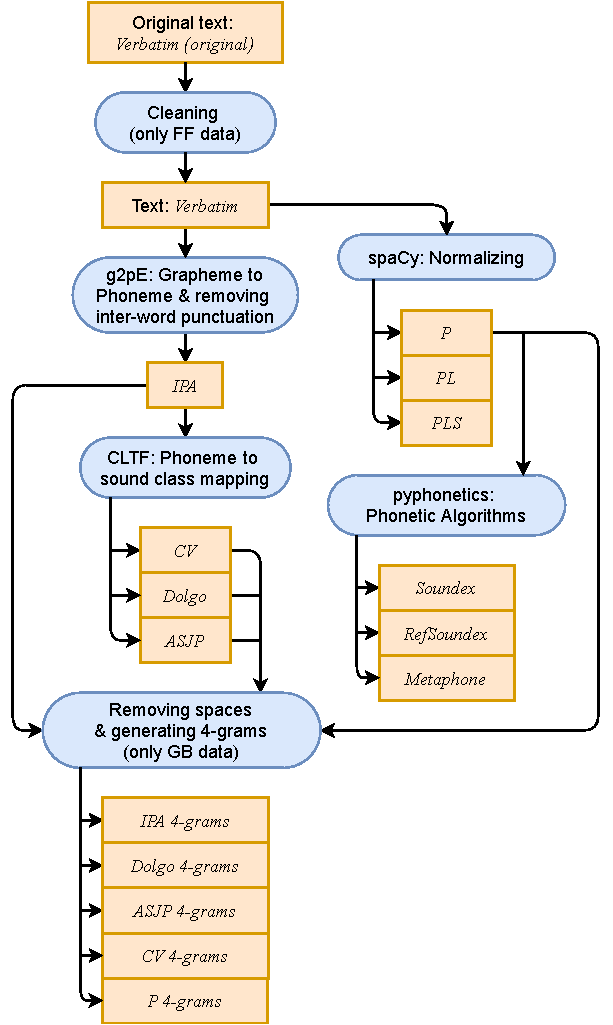
\includegraphics[width=0.7\textwidth]{figures/transcription}
  \caption{Transcription setup, orange = data, blue = process}
  \label{fig:transcription}
\end{figure}


% Statistical analysis
% Vocab reduction on some corpus
% Vocab size counting: Space Tokenize, count tokens that are not punctuation and are not numbers, upper- / lower-case is dismissed. This leaves soundex tokens in. Texts of a pair are concatenated
\section{Transcription Characteristics}
To better understand the characteristics of the phonetic transcription systems and the idiosyncrasies of the datasets, we conduct some preliminary investigations.
We calculate the vocabulary size scaling factor ($VSSF$) for each transcription system by determining the ratio of the number of distinct lexical types before and after transcribing.
A $VSSF$ of 1.5, for example, indicates that the transcription system examined increases the vocabulary size by 50\%.
This way, we can assess the granularity of the different transcription systems.
A vocabulary reduction of 50\%, for example, indicates that on average two words are binned into one transcription.
In practice, there may be some transcriptions grouping many words while many transcriptions would have a one-to-one mapping to a single word.
We calculate the absolute vocabulary size and the $VSSF$ per transcription system per dataset.
Table~\ref{tab:system_characteristics} shows the results.\\
First, let us take a look at findings for the Gutenberg dataset, which are visualized in figure~\ref{fig:vssf_transcriptions_gb}.
The $Verbatim$ text contains 50277 types.
Both $IPA$ and $ASJP$ increase the vocabulary size by a significant amount, 20.68\% and 11.21\% respectively.
This is to be expected as the alphabet of both systems is larger than the alphabet of verbatim text and thus more types can be generated.
The text with removed punctuation ($P$) retains the same amount of types as verbatim text because punctuation symbols are not counted towards the vocabulary size.
By further lemmatizing the texts ($PL$), more tokens are binned and the resulting vocabulary is reduced by 18.6\%.
Eliminating stop words ($PLS$) removes 220 more types.
The $Dolgo$ system has an even smaller amount of types, but still retains more type granularity than the more simple phonetic algorithms.
$RefSoundex$ and $Metaphone$ reduce the vocabulary size by 41.44\% and 47.29\% respectively.
Because of its length restriction to four characters, $Soundex$ can at most produce 8,918 unique types (A000 to Z666) with only 4250 of them appearing in the data.
Lastly, $CV$ reduces the number of types the most and retains only 1954 types.
A reduction to 3.89\% of the original vocabulary size implies that on average ca.\ 26 words are binned into one transcription.\\

\begin{figure}
  \centering
  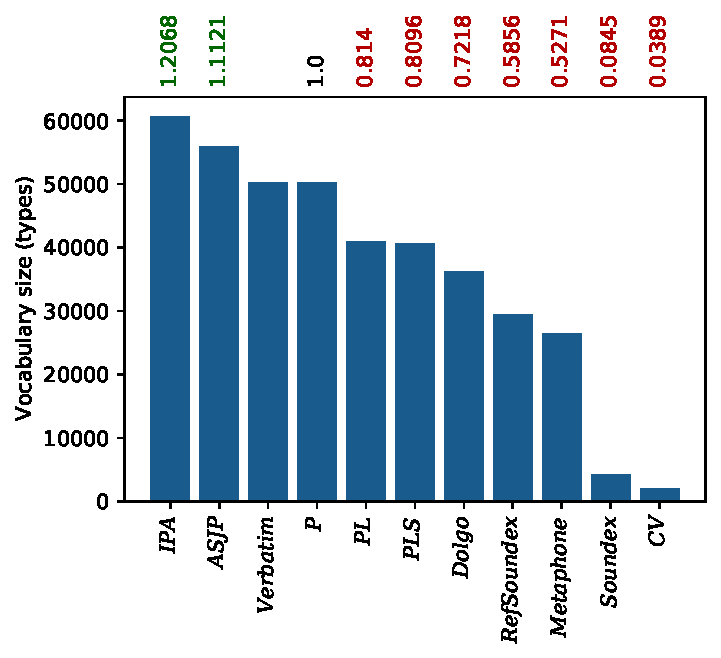
\includegraphics[width=0.7\textwidth]{figures/vocab_sizes_2021-07-28_14-42-08_gb_pt}
  \caption{Vocabulary sizes for transcriptions on Gutenberg dataset with $VSSFs$ above}
  \label{fig:vssf_transcriptions_gb}
\end{figure}
\begin{figure}
  \centering
  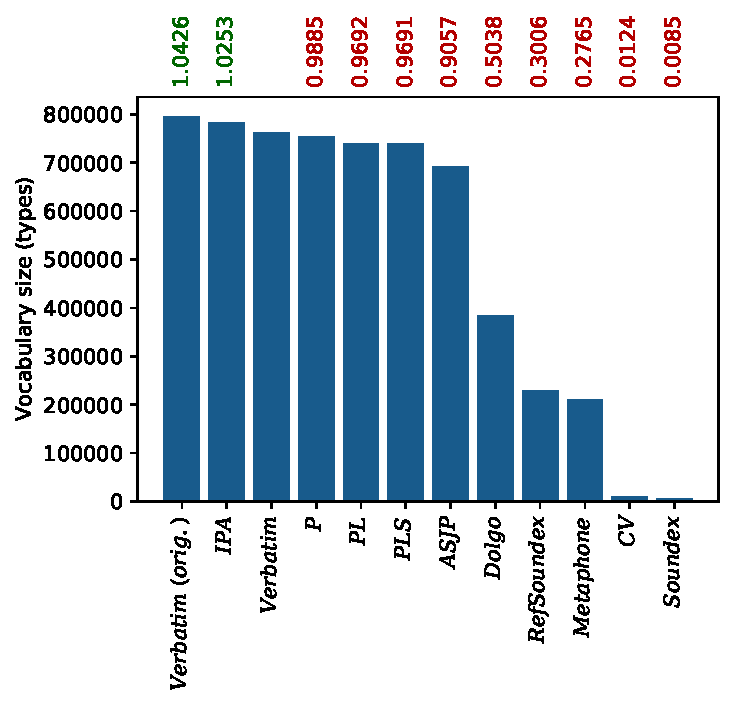
\includegraphics[width=0.7\textwidth]{figures/vocab_sizes_2021-07-27_16-57-38_ff_pt}
  \caption{Vocabulary sizes for transcriptions on Fan-fiction dataset with $VSSFs$ above}
  \label{fig:vssf_transcriptions_ff}
\end{figure}

Figure \ref{fig:vssf_transcriptions_ff} shows the results for the same analysis but using the Fan-fiction dataset.
Both plots are predominantly similar but exhibit a few interesting differences stemming from the characteristics of the transcription systems and the datasets.
Note that the Fan-fiction dataset is substantially larger than the Gutenberg dataset, also leading to a larger total vocabulary count.\\
First, the vocabulary size of the uncleaned (original) verbatim text is 4.26\% larger than that of the cleaned one.
This was expected as we removed certain words during cleaning.
Next, it can be observed that there is a difference between verbatim text and punctuation-removed text ($P$).
This may stem from the Fan-fiction dataset including many more different punctuation symbols which are removed to create the $P$ transcription but not when counting types in verbatim text.
Also, the relative difference between $P$ on the one hand and $PL$ as well as $PLS$ on the other is much smaller.
This could indicate that the Fan-fiction dataset has many out-of-vocabulary tokens that are not easily lemmatized.
Compared to the Gutenberg dataset, which consists of texts from published books, this would make sense as the acceptance criteria for Fan-fiction stories are much lower than those for books.
For the phonetic algorithms, $Soundex$ has a smaller vocabulary than $CV$.
As mentioned above, the codes generated by the $Soundex$ algorithm are bound to 4 characters in length.
Because $CV$ tokens are only restricted to a binary alphabet, but do not have any length restrictions, with a large enough text sample the $CV$ vocabulary outnumbers the $Soundex$ vocabular.
To substantiate this claim, we created a vocabulary list for each text pair in the Fan-fiction dataset.
Then we accumulated the vocabulary lists one by one to examine if the transcribed texts follow Heaps' Law.
Figure~\ref{fig:cumvocab_soundexcv} shows the sizes for the accumulated vocabulary for $Soundex$ and $CV$ when reading in the texts from the Fan-fiction dataset in a shuffled order.
The vocabulary of the $Soundex$ transcription grows fast in the beginning but then begins to max out at around 6000 types.
For the $CV$ transcription on the other hand, the accumulated vocabulary size grows slowly in the beginning, probably due to its restricted alphabet, but does not hit a ceiling and continues to grow beyond $Soundex$'s vocabulary size.\\
Arguably, the most notable difference is that when transcribing the Gutenberg dataset $ASJP$ leads to an increase in vocabulary size whereas using the Fan-fiction dataset $ASJP$ surprisingly results in a significant reduction of the vocabulary.
Note that as shown in figure~\ref{fig:transcription} $ASJP$ results from the $IPA$ transcription.
To attain a clearer view of what is happening here, we also calculate the accumulated vocabulary sizes for verbatim, $IPA$, $ASJP$, and $Dolgo$, shown in figure~\ref{fig:cumvocab_all}.
This plot poses two additional questions\footnote{Both phenomena persist when using single texts instead of text pairs for the cumulative vocabulary size analysis.}:
\begin{enumerate}
    \item Why is there a sudden change in curvature in the accumulated vocabulary size?
    \item Why do $IPA$ and verbatim text diverge on the left side but stay at a constant difference after the change in curvature on the right side?
\end{enumerate}
The first question has an obvious answer.
The Fan-fiction dataset is sorted.
The first half consists of only same-author pairs with all different-author pairs residing in the second half.
Table \ref{tab:dataset_authors} shows information on the author distribution of both datasets segmented into same-author and different-author parts.
With 47813 authors, the different-author part of the Fan-fiction dataset has around 7.47 times as many authors as the same-author part.
For the same-author part, on average one author wrote 1.036 individual texts whereas for the different-author part this number is 8.7022\footnote{Or in terms of dataset samples, on average authors contributed to 0.518 and 4.3511 text pairs respectively.}.
It comes as no surprise then that -- despite individual text and vocabulary sizes being nearly equal for both parts -- the vocabulary of the different-author part is much more diverse.
This diversity leads to the higher slope in the different-author part.
As a side note, the bias-mitigated Gutenberg dataset does not exhibit a change of curvature when analyzing it as above.
This is also reflected in the number of authors for the same- and different-author parts in table \ref{tab:dataset_authors}.
The number of authors for both parts are almost identical, and most authors appear in both parts.
Also, the number of texts an author contributed to the dataset is nearly equal between both parts.
We conclude that the number of authors is correlated to the vocabulary size of a given dataset.
Further investigations are necessary to determine whether the difference in author distribution and thus in vocabulary size in the Fan-fiction dataset has an effect on the results from the PAN20 task where this dataset was used.\\
As of yet, we do not have an answer for the second question.
To change the perspective of this phenomenon, figures~\ref{fig:cumvocab_same} and~\ref{fig:cumvocab_diff} show the cumulative vocabulary size for the same-author and different-author part in isolation.
As expected, all curves follow Heaps' Law and the total vocabulary of the same-author part is lower than that of the different-author part.
The surprising difference is that the curves for verbatim and $IPA$ in figure~\ref{fig:cumvocab_diff} do not diverge.
In contrast to the same-author part, for the different-author part the transcription to $IPA$ does \textit{not} lead to an increased vocabulary size.
We investigated some possible explanations of this phenomenon.
The samples from both parts are transcribed in one coherent process and also plotted in one go, lowering the probability of an implementation error.
The percentage of alphabet characters (a-zA-Z) in both parts is almost equal.
The only small difference we found is in the fraction of words that occur in the ASPELL dictionary.
For the same-author part 15\% of the words are in ASPELL while for the different-author part only 10\% are in ASPELL\@.\\
We suspect that the decrease in vocabulary size of $ASJP$ compared to verbatim text (fig.~\ref{fig:vssf_transcriptions_ff}) has two reasons.
First, the missing increase for the vocabulary size of $IPA$ in the different-author part.
As $IPA$ is the transcription preceding $ASJP$, the vocabulary size of the former directly impacts the that of the latter.
Second, in figure \ref{fig:cumvocab_same} we observe that $ASJP$ still produces a lower vocabulary count, even for the same-author part only.
This lets us speculate that some other factor, e.g., the quality of the dataset, must also play a roll in its transcription.
Maybe both, the same-author and the different-author part, are affected by the same phenomenon with the same-author part only slightly.
This hypothesis could be supported by comparing the vocabulary increase of $IPA$ between both datasets.
With the Gutenberg dataset, $IPA$ increases the vocabulary by 20.68\% (fig.~\ref{fig:vssf_transcriptions_gb}) while with the Fan-fiction dataset the vocabulary is only increased by 2.53\% (fig.~\ref{fig:vssf_transcriptions_ff}).
Still, this comparison should be interpreted cautiously because of the bespoken size differences of the datasets.
To this end, further investigation is needed.\\
Figure~\ref{fig:vssf_ngrams_gb} shows the vocabulary sizes for the $4$-grams, i.e., the amount of unique $4$-grams generated from each transcription of the Gutenberg dataset, compared to the vocabulary size of verbatim text.
With a binary alphabet, $CV$ creates only 16 unique $4$-grams.
This is followed by $Dolgo$, which could at most create 20736 $4$-grams of which 4061 appear in the data.
$ASJP$ increases upon the vocabulary count of verbatim text, as it has a bigger alphabet.
$4$-grams generated from punctuation-removed text have an even higher count.
This is due to intra-word punctuation not being removed and thus retaining many of the punctuation symbols from verbatim text.
Lastly, $IPA$ generates by far the most $4$-grams, as it has the biggest alphabet of all transcriptions used.


\begin{figure}
  \centering
  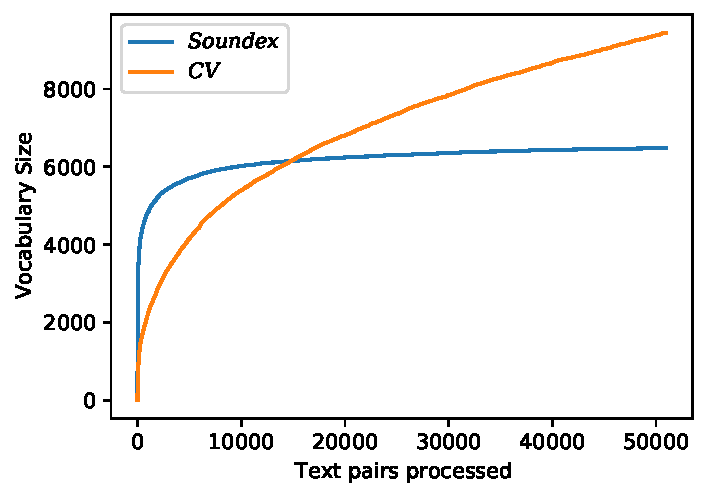
\includegraphics[width=0.7\textwidth]{figures/cum_vocab_size_ff_shuffled_soundexcv}
  \caption{Accumulated vocabulary size for $Soundex$ and $CV$, shuffled Fan-fiction dataset}
  \label{fig:cumvocab_soundexcv}
\end{figure}
\begin{figure}
  \centering
  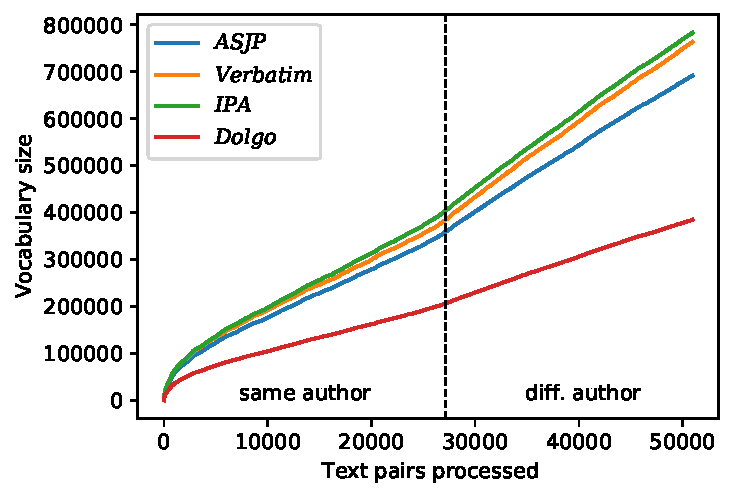
\includegraphics[width=0.7\textwidth]{figures/cum_vocab_size_ff_inorder_all}
  \caption{Accumulated vocabulary size for verbatim, $IPA$, $ASJP$, and $Dolgo$, in-order Fan-fiction dataset}
  \label{fig:cumvocab_all}
\end{figure}
\begin{figure}
  \centering
  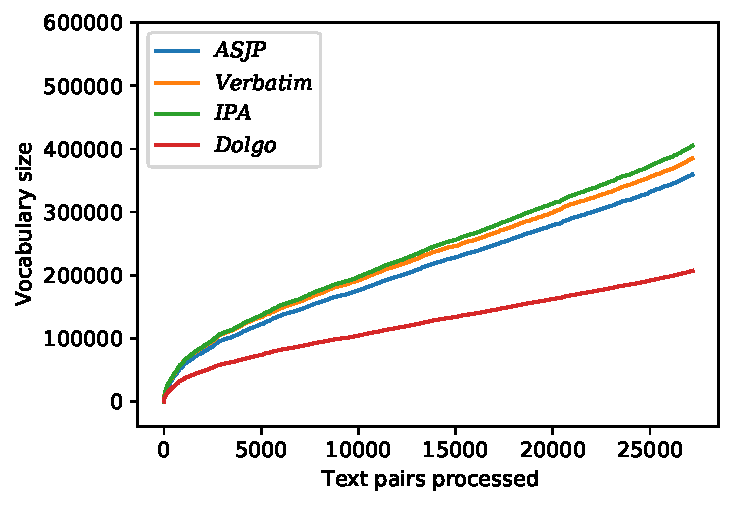
\includegraphics[width=0.7\textwidth]{figures/cum_vocab_size_ff_inorder_onlysame_ipa}
  \caption{Same-author part of accumulated vocabulary size for verbatim, $IPA$, $ASJP$, and $Dolgo$, in-order Fan-fiction dataset}
  \label{fig:cumvocab_same}
\end{figure}
\begin{figure}
  \centering
  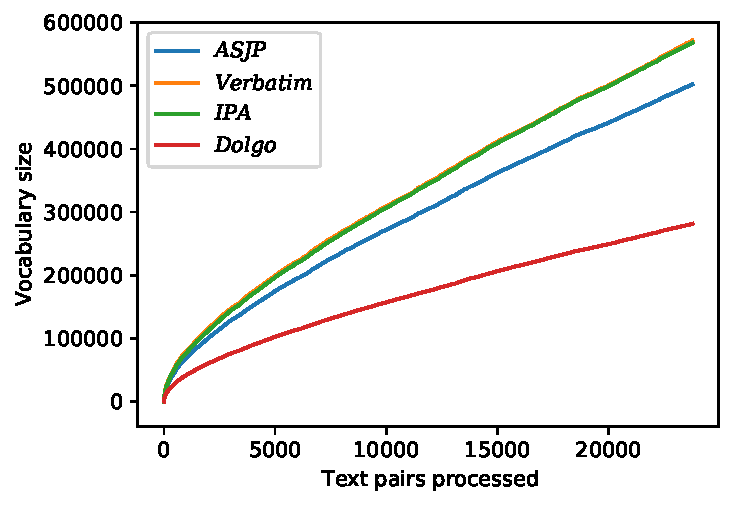
\includegraphics[width=0.7\textwidth]{figures/cum_vocab_size_ff_inorder_onlydiff_ipa}
  \caption{Different-author part of accumulated vocabulary size for verbatim, $IPA$, $ASJP$, and $Dolgo$, in-order Fan-fiction dataset.}
  \label{fig:cumvocab_diff}
\end{figure}

\begin{table}
\caption{Author distribution of the datasets used.}
\label{tab:dataset_authors}
\centering\small
\begin{tabular}{@{}l@{\hspace{1\tabcolsep}}lll@{}} % Use @{\hspace{2\tabcolsep}} to double the spacing
\toprule
\bf  & \bf Gutenberg & \bf Fan-Fiction \\
\midrule
\#authors in same-author part & 54 & 6397 \\
\#authors in different-author part & 56 & 47813 \\
\#authors in both parts & 53 & 1555 \\
Texts per author in same-author part & 4.8148 & 8.7022 \\
Texts per author in diff-author part & 4.7143 & 1.036 \\
\bottomrule
\end{tabular}
\end{table}


\newcommand{\specialcell}[2][c]{%
  \begin{tabular}[#1]{@{}c@{}}#2\end{tabular}}

\begin{table}
\caption{Characteristics of the transcription systems used. Verbatim represents plain English text. Verbatim (original) is the uncleaned version of the Fan-fiction dataset. Punctuation and whitespaces are not included in the alphabet size. Alphabet sizes are theoretically derived.}
\label{tab:system_characteristics}
\centering\small
\begin{tabular}{@{}l@{\hspace{1\tabcolsep}}rlrlr@{}} % Use @{\hspace{2\tabcolsep}} to double the spacing
\toprule
\bf System & \bf \specialcell{GB\\absolute} & \bf \specialcell{GB\\VSSF} & \bf \specialcell{FF\\absolute} & \bf \specialcell{FF\\VSSF} & \bf Alphabet size \\
\midrule
$Verbatim$ $(orig.)$ & -- & -- & 795621 & 1.0426 & 26(?) \\
$IPA$ & 60673 & 1.2068 & 782424 & 1.0253 & >100(?) \\
$ASJP$ & 55913 & 1.1121 & 691146 & 0.9057 & 41(?) \\
$Verbatim$ & 50277 & 1.0 & 763097 & 1.0 & 26(?) \\
$P$ & 50277 & 1.0 & 754293 & 0.9885 & 26(?) \\
$PL$ & 40924 & 0.814 & 739629 & 0.9692 & 26(?) \\
$PLS$ & 40704 & 0.8096 & 739530 & 0.9691 & 26(?) \\
$Dolgo$ & 36288 & 0.7218 & 384440 & 0.5038 & 11 \\
$RefSoundex$ & 29441 & 0.5856 & 229360 & 0.3006 & 36 \\
$Metaphone$ & 26501 & 0.5271 & 210973 & 0.2765 & 21 \\
$Soundex$ & 4250 & 0.0845 & 6471 & 0.0085 & 32 \\
$CV$ & 1954 & 0.0389 & 9436 & 0.0124 & 2 \\
$IPA$ $4$-$grams$ & 176092 & 3.5024 & -- & -- & 2 \\
$P$ $4$-$grams$ & 103983 & 2.0682 & -- & -- & 2 \\
$ASJP$ $4$-$grams$ & 78246 & 1.5563 & -- & -- & 2 \\
$Dolgo$ $4$-$grams$ & 4061 & 0.0808 & -- & -- & 2 \\
$CV$ $4$-$grams$ & 16 & 0.0003 & -- & -- & 2 \\
\bottomrule
\end{tabular}
\end{table}

\begin{figure}
  \centering
  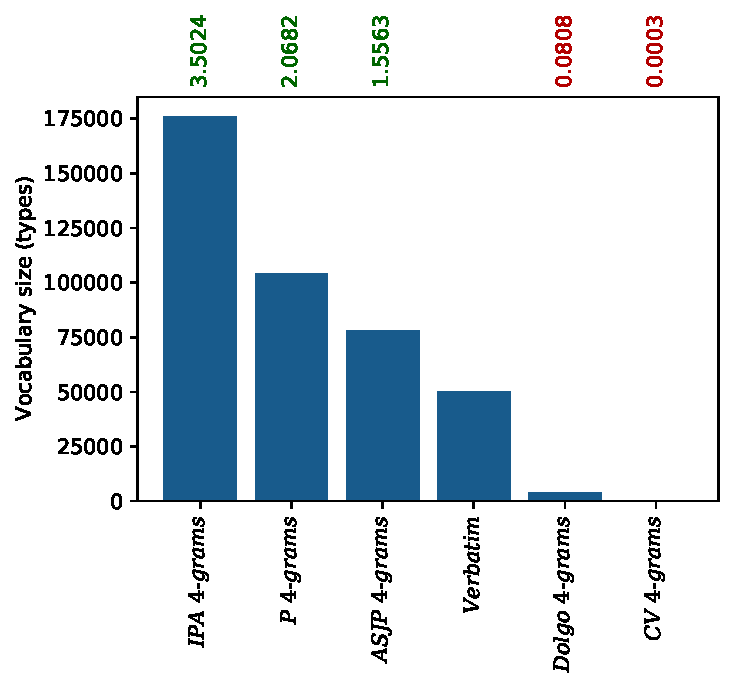
\includegraphics[width=0.7\textwidth]{figures/vocab_sizes_2021-07-28_14-42-08_gb_ngram}
  \caption{Vocabulary sizes for $4$-grams compared to verbatim.}
  \label{fig:vssf_ngrams_gb}
\end{figure}
\chapter{Experiments}\label{experiments}
As shown in figure~\ref{fig:process}, the main experimental setup can be structured into four parts.
In a preprocessing step, we standardize the Gutenberg dataset to the new PAN20 format and we clean the Fan-fiction dataset.
Then, we transcribe the datasets using the phonetic transcription methods defined earlier.
The resulting datasets, as well as the original dataset, are then used as the inputs to two widely used Authorship Verification algorithms which are described in more detail in this chapter.
For all experiments, we conduct three cross-validation runs with ten folds each.
We then average the results and compute the Bonferroni-corrected\footnote{As we conduct 30 runs on the same data, the likelihood of encountering a rare configuration that performs well and accepting it as statistically significant is high. Thus we divide the $p$-values for accepting statistical significance by 30.} statistical significance using a paired t-test as the test statistic.
Finally, we analyze the results.
\begin{figure}
  \centering
  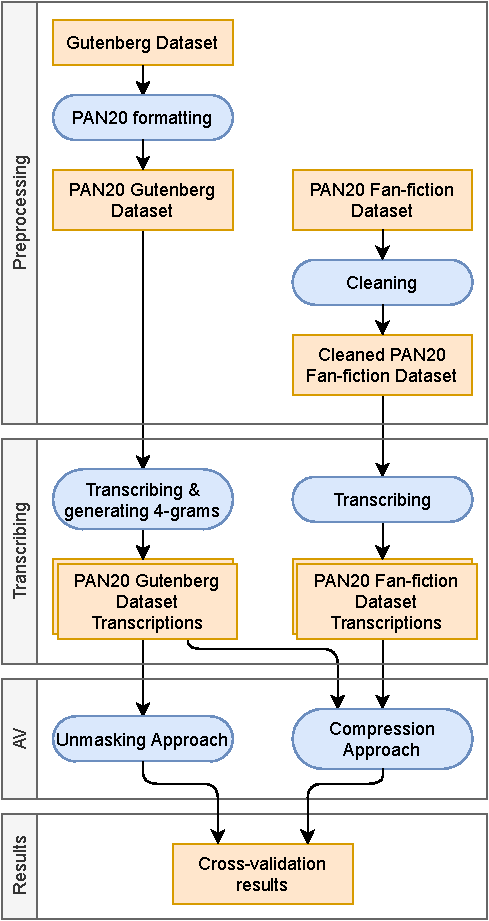
\includegraphics[width=0.6\textwidth]{figures/process}
  \caption{Experimental setup, orange = data, blue = process.}
  \label{fig:process}
\end{figure}

% 1.2 Compression Approach
\section{Compression Approach}\label{sec:compression-approach}
The first approach, used as a benchmark in PAN2020 and adapted to Authorship Verification from \cite{teahan2003compression}, uses a text compression method to determine the chance that two texts were written by the same author.
Text compression can be seen as encoding a given text with an encoding that is optimized for this text.
As discussed in \cite{brown1992upperBoundEntropy}, by determining this encoding, text compression can be used to estimate an upper bound to the entropy, i.e., the amount of information of characters in English text.
More specifically, by using the compression model optimized on some text A, the cross-entropy of encoding a text B with this model can be calculated.
During training, this is done for each pair in both directions.
The mean and average of the distance between the resulting cross-entropies are then used to train a logistic regression model.
The smaller the resulting difference, the more similar the texts, and the higher the chance that both are written by the same author.
The compression model used is Prediction by Partial Matching (PPM), a standard algorithm for lossless text compression, first introduced by \cite{cleary1984PPM}.
As done in PAN20, we employ an uncertainty interval of 5\%, i.e., predictions that are in the interval $[0.45, 0.55]$ are given a $non$-$answer$ classification.
The source code used is based on a reimplementation of the Authorship Attribution approach from \cite{teahan2003compression} as part of a reproducibility study in \cite{potthast2016reimplementation}.
The adaption for Authorship Verification stems from PAN20\footnote{\url{https://github.com/pan-webis-de/pan-code/tree/master/clef20/authorship-verification}}.
The source code extending the algorithm to use phonetic features and adding cross-validation functionality is available on GitHub\footnote{\url{https://github.com/torond/teahan03-phonetic}}.
% Add figure, only showing cross-validation side!

% 1.3 Unmasking Approach
\section{Unmasking Approach}\label{sec:unmasking-approach}
Unmasking was first introduced by \citeauthor{koppel2004unmasking} in 2004.
In short, it exploits the degradation of classifier accuracy when removing distinguishing features.
It turns out that iteratively removing those features leads to a faster degradation on text pairs by one author than on those by different authors.
Thus, the algorithm "unmasks" the text pairs and thereby reveals the information needed for classification.\\
% Formal definiton & explanation: unmasking step
This approach comprises two steps: First, a cross-validation method is employed to create the accuracy degradation curves for all training samples.
Secondly, a meta-classifier is trained on the resulting curves to differentiate between same-author and different-author curves.\\
%XXX From here on!
%For a given pair, the texts are seen to be created by two generative processes $p_1$ and $p_2$.
To compute a curve for a pair, both texts are chunked into parts longer than 500 words without splitting paragraphs.
The 250 words with highest average frequencies in the two texts are used as features.
In a 10-fold cross-validation, linear SVM models are trained to classify if a chunk belongs to the first or the second text.
The resulting accuracy is noted and the three most discriminating positive and negative features are removed from the feature set.
The cross-validation and feature removal are repeated until no features are left.\\
% meta-learning step
The set of curves is then used to train a linear SVM model as a meta-classifier.
As brought to the point by \cite{bevendorff2019unmaskingShortTexts}, features used are ``the curve points, the curves' point-wise first- and second-order derivatives, and the derivatives sorted by steepest point-wise drop''.\\
% Adaptation for short texts by Bevendorff et al., how is this different? Which features are actually being used?
Unmasking is one of the most robust Authorship Verification algorithms.
But as it requires sufficient chunks of no less than 500 words in length, it is only applicable for book-length texts.
To counter this, \cite{bevendorff2019unmaskingShortTexts} generalizes the algorithm to accommodate for short texts.
Chunks are generated by oversampling the bag-of-words pool of a given text.
Words from this pool are picked randomly without replacement until a length of 700 words is reached and the pool is reset afterwards.
In total, 30 chunks are generated, which are then used for curve generation as above, with the only exception that the five most positive and negative features are removed instead of only three.
As this approach introduces a significant amount of variance in the resulting curves, the unmasking step is repeated multiple times and the curves are averaged.
It is recommended to average at least 15--20 unmasking runs for each text pair.
In our experiments, we average the curves of 32 unmasking runs per text pair with varying chunk sizes of 500, 600, and 700 words respectively.
In the implementation supplied by \cite{bevendorff2019unmaskingShortTexts}\footnote{\url{https://github.com/webis-de/unmasking}} and used as the basis for our research, the meta-classifier uses the curves' ``central-difference gradients (first- and second-order), as well as their gradients sorted by magnitude''.
Also, the implementation predicts labels instead of confidence values, hence reducing F0.5u to F0.5\footnote{Weighting precision two times as much as recall, but not accounting for $non$-$answers$.} and C@1 to accuracy.
The source code extending the Unmasking framework for the use of phonetically transcribed datasets and implementing a cross-validation functionality is available on GitHub\footnote{\url{https://github.com/torond/unmasking}}.
Note that we only use the Gutenberg dataset for Unmasking as processing the larger Fan-fiction dataset for each transcription proved to be too time-intensive.
\chapter{Results}\label{results}
% Introduction: PAN20 uses these measures, so we do, too.
For the evaluation of our approaches we use several traditional as well as recently proposed measures.
\textcolor{olive}{(textbook citation needed for following definitions)} We use the convention that a pair is in the positive class iff both texts are written by the same author.
$tp$, $tn$, $fp$, $fn$ stand for the number of cases that where classified correctly as positive (true positives), correctly as negative (true negatives), falsely as positive (false positives) and falsely as negative (false negatives) respectively.\\
% Explain OOF cross-validation
% Precision
The \textbf{precision} $pre = \frac{tp}{tp+fp}$ of a classifier is the percentage of correct positive classifications $tp$ over all classifications $tp+fp$.
Thus, a precision approaching 1 indicates that an AV classifier's same-author predictions are near fully correct, meaning that there are nearly no false positives.\\
% Recall
The \textbf{recall} $rec = \frac{tp}{tp+fn}$ of a classifier is the percentage of correctly classified positive samples $tp$ over all positive samples $tp+fn$.
The lower the recall, the fewer same-author cases are recognized and predicted as such by an AV classifier.
In turn, a recall of 1 indicates that all same-author cases have been correctly identified.\\
% F1
Ideally, we want a system that classifies all same-author cases and only those as positive.
To measure this behavior, the \textbf{F1-score} $F_1 = 2\cdot\frac{prec\cdot{}rec}{prec+rec}$ can be used.
If both, precision and recall, approach 1 the F1-score of an AV classifier also approaches its maximum of 1.
Note that the F1 score weights precision and recall equally.
Especially for forensic Authorship Verification applications though, a high precision is more important than a high recall, as same-author decisions might be used as evidence and therefore must be reliable.
Also, in our setup, the F1 score ignores true negatives and therefore does not give an insight into how well the classifier detects different-author cases correctly.
For this, the different-author class would need to be assigned the positive label.\\
To mitigate some of the problems of the measures above and to better asses AV classifier performance, we use two more recently introduced measures.
% C@1, Point: non-answers (0.5) are possible
To measure include same-author and different-author classifications in the evaluation, one could use the accuracy $acc = \frac{tp+tn}{n}$, where $n = tp+tn+fp+fn$ is the total number of cases.
However, as \cite{bevendorff2019unmaskingShortTexts} points out, the results are often uncertain.
Also, in real-world applications wrong answers might be worse than non-answers.
Therefore, to give classification systems the option to withhold answers for difficult-to-decide cases, we use the \textbf{c@1-score} introduced by \cite{penas2011c_at_1} and adopted by PAN.
It is defined as $c@1 = \frac{n_{ac}}{n}+\frac{n_{ac}}{n}\cdot{}\frac{n_u}{n} = \frac{1}{n}\cdot{}\left(n_{ac}+\frac{n_{ac}}{n}\cdot{}n_u\right)$ where $n$ is again the total number of cases, $n_{ac} = tp+tn$ is the number of accurately classified cases and $n_u$ is the number of undecided cases.
This way, undecided cases count towards the c@1-score as if they were answered with the accuracy of the decided cases.
When an AV classifier gives an answer to all cases, the C@1-score is reduced to the accuracy.
A system that leaves all cases unanswered, receives a score of 0.\\
% F0.5u
Lastly, we use the \textbf{F0.5u-score} introduced by \cite{bevendorff2019unmaskingShortTexts}.
It is defined as $F_{0.5u} = \frac{(1+0.5^2)\cdot{}n_{tp}}{(1+0.5^2)\cdot{}n_{tp}+0.5^2\cdot{}(n_{fn}+n_u)+n_{fp}}$.
As mentioned above, a high precision result is more robust than a high recall one.
To account for this, the F0.5u-score weights precision two times as much as recall.
In addition, it also allows the classifiers to give non-answers.
However, as unanswered cases are often not useful in real-world applications, it interprets them as wrong answers.
Thus, the F0.5u-score highly emphasizes on the precision of an AV classifier.\\

% PAN20 measures:     AUC, C@1, F0.5u, F1, overall
% Unmasking measures: Precision, Recall, C@1, F0.5u
\textcolor{violet}{
TBD: Show and analyze results\\
}

% First: Gutenberg
% ->
%- For GB Unmasking: Argue 32 runs for stable results. This still only creates 262 curves. Show which parameters where used for those 32 runs
Before analyzing the final results, let us take a look at the sets of the degradation curves that resulted from Unmasking
% 4 gram curves fall much quicker! Show them! -> Rather run again with better window.


% Then: Fan-fiction


% FF
As cleaning step is phonetically informed we'll use verbatimorignal for comparing.

For r values higher than 0.05, prec rec higher, f05u cat1 lower.
Throwing out cases, prec rec f1 only consider cases where classifier is more sure about the result.


% GB
For CV, CV 4-grams, and Dolgo 4-grams the dataset is too small and all samples are predicted to be false, thus, Precision and Recall are ill-defined (zero division) and we'll leave these out.
Removed because ill-defined: 'cv', 'cv_4grams', 'dolgo_4grams', 'punct_4grams', 'dolgo', 'asjp_4grams', 'refsoundex', 'soundex'

% Also: Remember to answer the questions from the Introduction


% Compare to other approaches from PAN20
%As indicated earlier, through cross validation, we can use the entire data set for training and for testing, thus milking it in the most effective way. hehe, correction lolol.
% Note Gutenberg dataset is really small


In the following, we will discuss a number of possible reasons for the overall negative trend that phonetic transcriptions bring to the results.\\
Converting graphemes to phonemes, in our case verbatim text to its $IPA$ transcription, is a difficult task.
Moreover, when transcribing automatically, the transcription algorithm does not have any information about the pronunciation of the speaker of a given text.
Thus, usually text is transcribed to either the General (North) American pronunciation or the Received Pronunciation\footnote{British English}.
We use g2pE by \cite{kyubyong2019g2pE} which employs the Carnegie Mellon University Pronouncing Dictionary to look up transcriptions for words.
The CMU dictionary uses North American English as its pronunciation standard.
Thus, by transcribing we assume that the author has a North American English phonetic preference.
Transcribing, for example, both an Irish author's and a Nigerian author's texts to American English, one can imagine that a lot of phonetically relevant information, that could be used to distinguish them, is lost.
In the same vein, authors might \textit{actively} make efforts to impart certain phonetic qualities into their texts that are based on topic rather than the author's unconscious phonetic preference.
This becomes especially clear when an author uses direct speech, which often occurs in the datasets we use as they are both based on sets of fictional stories.
The ``voice in the author's head'' when writing a direct speech passage presumably varies greatly depending on the traits of the character depicted in the story.
Thus, extracting these features might aid in topic or genre identification more so than in Authorship Verification.
To mitigate this, direct speech could be removed from text entirely.\\
Another limitation of phonetic transcriptions for Authorship Analysis is due to the low-level nature they work at.
An authors' freedom of self-expression is limited on the sub-segmental level, i.e., concerning individual sounds.
Usually, the meaning of a word changes together with its pronunciation.
The only words for which this is not the case are synonyms such as the words "begin" and "start".
Thus, authors that want to express similar ideas arguably will sound similar on the sub-segmental level not because of their phonetic preference but due to the proximity of the topics.
More importantly, if authors want to express different ideas the resulting transcriptions will also be different, without the Authorship Verification classifier knowing if this difference stems from two unique authors with varied phonetic preferences or from one author discussing different topics.
Supra-segmental features such as stress or prose can be utilized more freely and might give a more informative base for Authorship Analysis.\\
Lastly and perhaps most importantly, standard Unmasking without using $n$-grams works on the lexical level, i.e., it uses entire words as atomic units and ignores the information encoded by the symbols inside a word.
With the step of transcription, however, we are precisely attempting to enhance this inner-word information.
Thus, for Unmasking the transcription of data serves only as a phonetically-informed binning method for types.
To mitigate this, we tried to use an $n$-gram based transcription method, with XXX results.\\



Describe n-gram effects of pt!


% Problem 3 / Following thoughts: Phonetic transcriptions / features are probably bad Authorship predictors but better predictors for other features such as genre, topic, age of setting.
\begin{table}
\caption{Significance of changes for Unmasking using the Gutenberg dataset, bonferroni-corrected.\\$=$: not statistically significant ($p \geq 0.05$)\\$*$: statistically significant ($p < 0.05$)\\$*\, *$: very statistically significant ($p < 0.01$)\\$***$: highly statistically significant ($p < 0.001$)}
\label{tab:p_unmasking_gb}
\centering\small
\begin{tabular}{@{}l@{\hspace{1\tabcolsep}}cccccccc@{}} % Use @{\hspace{2\tabcolsep}} to double the spacing
\toprule
\bf System & \bf Precision & \bf Recall & \bf F1 & \bf F0.5u & \bf c@1 \\
\midrule
$IPA$ & $=$ & $=$ & $=$ & $=$ & $=$ \\
$ASJP$ & $=$ & $=$ & $=$ & $=$ & $=$ \\
$Dolgo$ & $=$ & $=$ & $=$ & $=$ & $=$ \\
$RefSoundex$ & $=$ & $=$ & $=$ & $*\, *$ & $=$ \\
$Metaphone$ & $=$ & $=$ & $*$ & $*\, *$ & $*\, *$ \\
$Soundex$ & $=$ & $=$ & $=$ & $*\, *$ & $=$ \\
$CV$ & $*\, *$ & $=$ & $*\, *$ & $***$ & $***$ \\
$IPA$ $4$-$grams$ & $*\, *$ & $=$ & $*\, *$ & $***$ & $***$ \\
$ASJP$ $4$-$grams$ & $=$ & $=$ & $=$ & $=$ & $=$ \\
$P$ $4$-$grams$ & $=$ & $=$ & $=$ & $*$ & $*$ \\
$Dolgo$ $4$-$grams$ & $=$ & $=$ & $=$ & $***$ & $*\, *$ \\
$CV$ $4$-$grams$ & $*\, *$ & $=$ & $*\, *$ & $***$ & $***$ \\
$P$ & $=$ & $=$ & $=$ & $=$ & $=$ \\
$PL$ & $=$ & $=$ & $=$ & $=$ & $=$ \\
$PLS$ & $=$ & $=$ & $=$ & $=$ & $=$ \\
\bottomrule
\end{tabular}
\end{table}

\begin{table}
\caption{Significance of changes for the compression approach using the Fan-fiction dataset compared to verbatim text (uncleaned), $r=0.05$, bonferroni-corrected.}
\label{tab:p_teahan_ff}
\centering\small
\begin{tabular}{@{}l@{\hspace{1\tabcolsep}}ccccccc@{}} % Use @{\hspace{2\tabcolsep}} to double the spacing
\toprule
\bf System & \bf Precision & \bf Recall & \bf F1 & \bf F0.5u & \bf c@1 \\
\midrule
$Verbatim$ $(cleaned)$ & $***$ & $*\, *$ & $***$ & $***$ & $***$ \\
$IPA$ & $***$ & $***$ & $***$ & $***$ & $***$ \\
$ASJP$ & $*\, *$ & $***$ & $***$ & $=$ & $***$ \\
$Dolgo$ & $***$ & $***$ & $***$ & $***$ & $***$ \\
$RefSoundex$ & $***$ & $***$ & $***$ & $***$ & $***$ \\
$Metaphone$ & $***$ & $***$ & $***$ & $***$ & $***$ \\
$Soundex$ & $***$ & $***$ & $***$ & $***$ & $***$ \\
$CV$ & $***$ & $*\, *$ & $***$ & $***$ & $***$ \\
$P$ & $***$ & $***$ & $***$ & $***$ & $***$ \\
$PL$ & $***$ & $***$ & $***$ & $***$ & $***$ \\
$PLS$ & $***$ & $***$ & $***$ & $***$ & $***$ \\
\bottomrule
\end{tabular}
\end{table}


\begin{table}
\caption{Significance of changes for the compression approach using the Gutenberg dataset compared to verbatim text, $r=0.05$, bonferroni-corrected.}
\label{tab:p_teahan_gb}
\centering\small
\begin{tabular}{@{}l@{\hspace{1\tabcolsep}}ccccccc@{}} % Use @{\hspace{2\tabcolsep}} to double the spacing
\toprule
\bf System & \bf Precision & \bf Recall & \bf F1 & \bf F0.5u & \bf c@1 \\
\midrule
$IPA$ & $=$ & $*$ & $*$ & $=$ & $***$ \\
$ASJP$ & $=$ & $=$ & $=$ & $=$ & $***$ \\
$Metaphone$ & $**$ & $=$ & $=$ & $**$ & $***$ \\
$IPA$ $4$-$grams$ & $=$ & $=$ & $=$ & $***$ & $***$ \\
$P$ & $=$ & $=$ & $=$ & $=$ & $***$ \\
$PL$ & $=$ & $=$ & $=$ & $**$ & $***$ \\
$PLS$ & $=$ & $=$ & $*$ & $=$ & $=$ \\
\bottomrule
\end{tabular}
\end{table}
\chapter{Conclusion}\label{conclusion}
% Short summary
\textcolor{violet}{
TBD: Summary, conclusion, outlook
}

Conclude from end of last section: (Maybe throw out direct speech), use supra-segmental features, use more character-based methods.

%Care has been taken to make all research easily reproducible and understandable (source-code READMES etc.).

% Discussion
% Initially suspected no improvement with transcription approaches. Probably too much information is lost in transcribing.
% Where to put this?


%Outlook:\\
%- Improve usability of unmasking, cite DH paper (Juola 2007), got a request for use of unmasking
%- Use large PAN20 dataset on better hardware.
%- Closer inspection of possible correlation: vocab size ~ evaluation results
%- Down-sample transcriptions so that vocab size is the same.
%- Feature set analysis, what martin said.
%- Use more clever methods that infer meaning by phonetic markers, e.g., intonation (questions with "?")


% "Clever Features"
% - n-gram approach instead of word-tokenization
% - phonetic richness / complexity (over time)
% - vowel-phoneme over time
% - sound-classes over time (e.g. hard sounds / plosives compared to soft sounds)
% - sound classes: consonants and place of articulation (e.g. labial, nasal, ...)

% Bibliography
\bibliographystyle{apalike} % plainnat requires package natbib. An alternative is apalike
\bibliography{literature}    % load file literature.bib

\end{document}

